\documentclass[11pt,a4paper]{article}

\usepackage[T1]{fontenc}
\usepackage{amsmath,amssymb,amsthm}
\usepackage{graphicx}
\usepackage{booktabs}
\usepackage[margin=2.4cm]{geometry}
\usepackage[hidelinks]{hyperref}

\theoremstyle{plain}
\newtheorem{theorem}{Theorem}[section]
\newtheorem{proposition}[theorem]{Proposition}
\newtheorem{corollary}[theorem]{Corollary}
\newtheorem{conjecture}[theorem]{Conjecture}
\theoremstyle{definition}
\newtheorem{definition}[theorem]{Definition}
\newtheorem{remark}[theorem]{Remark}

\newcommand{\ZZ}{\mathbb{Z}}
\newcommand{\RR}{\mathbb{R}}
\newcommand{\Nn}{\mathbb{N}}
\newcommand{\pp}{\mathrm{p}}
\newcommand{\Ind}{\operatorname{In}}
\DeclareMathOperator{\mob}{mob}

\title{\bfseries Inertia Exponents of Graphs: Boolean Admissibility,\\
the \texorpdfstring{$q/s$}{q/s} Ceiling, and a Conjectured Barrier at $3$}
\author{}
\date{}

\begin{document}
\maketitle

\begin{abstract}
How large can the number of positive eigenvalues of an adjacency matrix be, relative to
the number of negative ones?  Elphick, Kumar, Pragada and Spier (2026) reduce this to a
purely algebraic question: find \emph{$(q,s)$-admissible} Boolean polynomials, i.e.\ 
multilinear $P\in\ZZ[x_1,\dots,x_q]$ whose Moebius coefficients $c_T$ are non-negative
above level $s$ and satisfy $c_{[q]}>0$; each such $P$ yields graphs with
$n^+=\Theta\big((n^-)^{q/s}\big)$, so the largest attainable exponent $q/s$ governs the
problem, and Mohar's question is equivalent to whether that exponent is bounded.  We
give an exact reformulation of admissibility as feasibility of a $2^q-1$-variable
$0$--$1$ linear program, which turns an opaque polynomial search into a certified
combinatorial computation.  Using it we determine $s_{\min}(q)$, the smallest admissible
level, exactly for $q\le 7$; we prove that $s=1$ forces $q=2$, with the unique witness
$(1-x_1)(1-x_2)$; and we certify exact characteristic polynomials and inertia of the
graphs we construct, with no floating point in any certificate.  The certified data and
a targeted heuristic search give no admissible pair with $q\ge 3s$, which we conjecture
to be a genuine barrier: if true, $n^+<O\big((n^-)^3\big)$ uniformly, answering a
question of Elphick--Kumar--Pragada--Spier positively.  We do \emph{not} prove it.
\end{abstract}

\section{Introduction}

Let $G$ be a finite simple graph of order $n$ with adjacency matrix $A(G)$, and write
$\Ind(G)=(n^+(G),n^0(G),n^-(G))$ for the numbers of positive, zero and negative
eigenvalues of $A(G)$, counted with multiplicity.  The \emph{positive inertia index}
$\pp(G)=n^+(G)$ and its negative counterpart $n^-(G)$ are classical invariants; for
strongly regular graphs they are tied to the absolute bound of Delsarte, Goethals and
Seidel by an elementary argument (see \S\ref{sec:related}).

A natural question is how large $\pp(G)$ can be relative to $n^-(G)$.  Two naive answers
are both wrong.
\begin{itemize}
\item[(i)] $\pp(G)\le n-1$ is true but useless: it ignores $n^-$.  Akbari, Elphick,
      Kumar, Pragada and Tang conjectured the much stronger
      $\pp(G)\le \binom{n^-(G)+1}{2}$, generalizing the absolute bound to all graphs.
      This is \emph{false}: the family $W(k)$ of Charles--Farber--Johnson--Kennedy-Shaffer,
      rediscovered by Chen and Li, has $n^-(W(k))=k-1$ and $\pp(W(k))=\binom{k}{2}+1$, so
      the conjecture is exceeded by exactly $2$.
\item[(ii)] Conversely, graphs with very few negative eigenvalues can have $\pp(G)\to\infty$
      fast.  Elphick, Kumar, Pragada and Spier constructed non-singular graphs with
      $n^-=k$ and $\pp=\Omega(k^{7/3})$, which resolved Mohar's question (is the order of a
      graph with $k$ non-positive eigenvalues $O(k^2)$?) in the negative, and refuted the
      conjecture in (i).
\end{itemize}
Elphick--Kumar--Pragada--Spier also isolate a clean remaining question: is there a
polynomial $f$ with $\pp(G)\le f(n^-(G))$ for every graph $G$?  The only upper bound known
for $\pp$ in terms of $n^-$ is exponential.

\subsection*{The algebraic engine}

Their reduction is the right starting point.  Let $q\ge 1$.  A \emph{multilinear
polynomial} is
\[
P(x_1,\dots,x_q)=\sum_{T\subseteq[q]} c_T\prod_{i\in T}x_i,\qquad c_T\in\ZZ ,
\]
with $[q]=\{1,\dots,q\}$; write $1_S$ for the indicator vector of $S\subseteq[q]$.  $P$
is \emph{Boolean} if $P(x)\in\{0,1\}$ for every $x\in\{0,1\}^q$, equivalently if
$g(S):=P(1_S)\in\{0,1\}$ for all $S$.

\begin{definition}[$(q,s)$-admissibility \cite{ElphickEtAl2026Inertia}]
\label{def:adm}
$P$ is \emph{$(q,s)$-admissible} if it is Boolean and
\begin{enumerate}
\item[(a)] $P(1,\dots,1)=g([q])=0$;
\item[(b)] $c_{[q]}>0$;
\item[(c)] $s=\max\{\,|T|:\ c_T<0\,\}$, so $c_T\ge 0$ for all $|T|>s$.
\end{enumerate}
\end{definition}

Elphick--Kumar--Pragada--Spier prove that such a $P$ produces graphs of order $m^q$ with
$\pp=\Theta(m^q)$, $n^-=\Theta(m^s)$, $n^0=0$; hence $\pp=\Theta\big((n^-)^{q/s}\big)$.
Their explicit $(7,3)$ example yields the exponent $7/3$; they report, without exhibiting
it, a $(32,12)$ example yielding $8/3$.

\subsection*{What we do}

\begin{itemize}
\item[\textbf{(A)}] We give an exact reformulation of \textup{Def.~\ref{def:adm}} as
      feasibility of a $2^q-1$-variable $0$--$1$ linear program
      (Prop.~\ref{prop:ref}).  Admissibility becomes a question about the Moebius
      transform of a $\{0,1\}$-valued function, and level feasibility is monotone in $s$
      and in $q$, which certifies binary search and makes infeasibility claims checkable
      (Props.~\ref{prop:level0}--\ref{prop:monotone}).
\item[\textbf{(B)}] \textbf{A complete small case.}  We prove that $s=1$ forces $q=2$,
      with the unique witness $(1-x_1)(1-x_2)$
      (Thm.~\ref{thm:s1}).  This also shows $\pp(G)\le \Theta\big((n^-)^{2}\big)$ cannot be
      improved by ``degenerate'' admissibility.
\item[\textbf{(C)}] \textbf{Exact data.}  We determine $s_{\min}(q)$ exactly for
      $q=2,\dots,7$, namely $1,2,2,3,3,3$ (Thm.~\ref{thm:cert}), each with a
      machine-checkable witness and a MILP infeasibility certificate.
\item[\textbf{(D)}] \textbf{Exact certificates.}  For every construction we verify the
      closed-form spectrum three ways: exact trace moments
      $\operatorname{tr}A^k=\sum_T\lambda_T^k(m-1)^{|T|}$, exact characteristic
      polynomial, and exact inertia computed from exact algebraic roots.  No floating
      point enters any certificate.
\item[\textbf{(E)}] \textbf{A conjectured barrier.}  Conjecture~\ref{conj:barrier}: every
      admissible pair satisfies $q<3s$.  If true, $\pp(G)=O\big((n^-(G))^{3}\big)$
      uniformly, answering the open question of Elphick--Kumar--Pragada--Spier positively.
      We give certified support for $q\le 7$ and report honestly that we have not proved
      it and found no counterexample.
\end{itemize}

\section{Related work}
\label{sec:related}

\paragraph{Inertia indices.}  $n^+$ and $n^-$ are studied in the classical spectral
literature \cite{CvetkovicDoobSachs1980,BrouwerHaemers2012}.  Ma, Yang and Li
\cite{MaYangLi2013} and Fan and Wang \cite{FanWang2017} give bounds in terms of the
matching number and cyclomatic number.  Xu, Zhen and Wong \cite{XuZhenWong2024} relate
$n^-$ to girth and diameter.

\paragraph{Strongly regular graphs and the absolute bound.}  For a primitive strongly
regular graph with spectrum $d^{(1)},r^{(f)},s^{(g)}$, the absolute bound
$2n\le g(g+3)$ \cite{DelsarteGoethalsSeidel1978} reads $2\pp\le n^-(n^-+1)$ because
$\pp=f+1$, $n^-=g$.  This is the observation that led to Conjecture 1.1 of
\cite{AkbariEtAl2026}, now refuted.

\paragraph{Torga{\v{s}}ev's function.}  Torga{\v{s}}ev proved that for each $k$ there are
finitely many \emph{reduced} graphs (no isolated vertices, no twins) with $n^-=k$
\cite{Torgasev1985a}, and computed the maximum of $n^+$ over reduced graphs for $k=1,2,3$
\cite{Torgasev1985b,Torgasev1989,Torgasev1992}.  The first open value is $k=4$; Chen and
Li \cite{ChenLi2026} exhibit a reduced graph with $n^-=4$, $n^+=11$, and Elphick et
al.\ report $f(4)\ge 11$.  Kotlov and Lov\'asz \cite{KotlovLovasz1996} bound the order in
terms of the rank, and Barrett et al.\ \cite{BarrettEtAl2014} provide the linear-algebra
tool (a rank-$r$ real symmetric matrix has a non-singular principal submatrix of order
$r$) used by Elphick et al.\ to pass between $n^-$ and $n^-+n^0$.

\paragraph{The reduction in use.}  Elphick, Kumar, Pragada and Spier
\cite{ElphickEtAl2026Inertia} show that a $(q,s)$-admissible polynomial gives graphs with
$\pp=\Theta((n^-)^{q/s})$ using the non-complete extended $P$-sum (NEPS) of Cvetkovi\'ic
\cite{Cvetkovic1971,CvetkovicSimic1993}.  Their Theorem 3.1 is the engine we use;
\S\ref{sec:spectrum} gives a self-contained proof together with the exact eigenvalue
formula.  Their $(7,3)$ polynomial is the starting point for our computations and we
re-verify it independently.  Francis and Uptain \cite{FrancisUptain2026} refute a
companion conjecture on line graphs.

\section{Preliminaries}

\subsection{Moebius transform on the Boolean lattice}

Identify $S\subseteq[q]$ with the subcube of $\mathbb R^q$ of vectors vanishing outside
$S$.  For $u\subseteq[q]$, let
\[
D(u)\,=\,\sum_{v\subseteq u}(-1)^{|u|-|v|}\,v .
\]
Then for any function $g:2^{[q]}\to\ZZ$ there is a unique function $c$ with
$c(u)=D(u)\,g$, and
\begin{equation}
\label{eq:zeta}
\sum_{T\subseteq S}c(T)=\sum_{T\subseteq S}D(T)\,g=g(S)\qquad\text{for all }S\subseteq[q].
\end{equation}
So $g$ and $c$ are mutually inverse zeta/Moebius transforms on the Boolean lattice.  If
$c$ are the coefficients of a multilinear $P$, then $g(S)=P(1_S)$, so \textup{(A)} says:
\emph{$P$ is $(q,s)$-admissible iff the zeta/Moebius pair $(c,g)$ satisfies
$g\in\{0,1\}^{2^{[q]}}$, $g([q])=0$, $c([q])\ge 1$, and $c(T)\ge 0$ for $|T|>s$.}

\subsection{The graph operation}
\label{sec:neps}

For a graph $H$ on vertex set $X(H)$ let $I_H$ be its identity and $J_H$ the all-ones
matrix.  Given graphs $G_1,\dots,G_q$ and a basis
$\mathcal B\subseteq\{0,1\}^q\setminus\{0\}$, the NEPS graph
$\mathrm{NEPS}(G_1,\dots,G_q;\mathcal B)$ has vertex set $\prod_i X(G_i)$ and joins
$(u_1,\dots,u_q)$ to $(v_1,\dots,v_q)$ whenever for some
$b=(b_1,\dots,b_q)\in\mathcal B$ we have $u_i=v_i$ if $b_i=0$ and
$u_iv_i\in E(G_i)$ if $b_i=1$.  Its adjacency matrix is the sum of tensor products
\[
A=\sum_{b\in\mathcal B} A(G_1)^{b_1}\otimes\cdots\otimes A(G_q)^{b_q},
\qquad A(H)^0=I_H,\quad A(H)^1=A(H).
\]
For $G_i=K_m$ we have $A(K_m)=J_m-I_m$.

Let $P$ be Boolean, put
\[
\mathcal F=\{S\subseteq[q]:P(1_{[q]\setminus S})=1\},\qquad
\mathcal B=\{\mathbf 1_S:S\in\mathcal F\},
\]
and let $G_m:=\mathrm{NEPS}(K_m,\dots,K_m;\mathcal B)$ ($q$ factors).  Since
$P(\mathbf 1)=0$ we get $\mathbf 0\notin\mathcal B$ when $P$ is $(q,s)$-admissible, and
$|V(G_m)|=m^q$.

\subsection{Inertia and non-positive subspaces}
\label{sec:dictionary}

We use two standard facts.  \emph{(F1)} For a real symmetric $A$, the number of strictly
positive eigenvalues equals $\max\{\dim W: x^{\mathsf T}Ax>0 \text{ for all } x\in
W\setminus\{0\}\}$ (Sylvester's law of inertia, \cite{HardyLittlewoodPolya1952}), hence
equals $\min\{\dim S: x^{\mathsf T}Ax\le 0 \text{ for all } x\in S^\perp\}$.
\emph{(F2)} Courant--Fischer: $\lambda_k=\min_{\dim S\,=\,k-1}\max_{x\perp S}
\frac{x^{\mathsf T}Ax}{x^{\mathsf T}x}$ \cite{CourantFischer1927,Hoffman1947}.

One motivational remark.  Writing $q_G(x)=\sum_{uv\in E(G)}x_ux_v$, fact (F1) says
$\pp(G)=\min\{\dim S: q_G\le 0 \text{ on } S^\perp\}$, so a large positive inertia forces
\emph{every} subspace on which $q_G$ is non-positive to be small.  For an independent set
$I$, the span of $\{e_i: i\in I\}$ is non-positive for $q_G$; by Courant--Fischer with
$S=\operatorname{span}\{e_v: v\notin I\}$ one gets $\lambda_{n-\alpha(G)+1}(G)\le 0$
and hence
\[
\pp(G)\le n-\alpha(G)=\tau(G). \tag{1}
\]
This elementary bound is attained by $C_5$ ($\pp=3$, $\alpha=2$) and is a useful sanity
check on any candidate construction.  It is not the subject of this paper, which asks a
finer question: how large $\pp$ can be when $n^-$ is prescribed.

\section{The reformulation}
\label{sec:ref}

\begin{proposition}[exact linearisation]
\label{prop:ref}
Fix $q\ge 1$ and $s\ge 1$.  There exists a $(q,s)$-admissible polynomial if and only if
the following $0$--$1$ linear program is feasible in the $2^q-1$ binary variables
$g(S)$ ($S\subseteq[q]$, $S\neq[q]$):
\[
\sum_{S\subseteq[q]}(-1)^{q-|S|}\,g(S)\ \ge\ 1, \tag{L0}
\]
\[
\sum_{S\subseteq T}(-1)^{|T|-|S|}\,g(S)\ \ge\ 0
\qquad\text{for all }T\subseteq[q],\ T\neq[q],\ |T|>s. \tag{L1}
\]
Moreover, for any feasible $g$ the value $s'=\max\{|T|: c(T)<0\}$ satisfies $s'\le s$,
and $s'=s$ for some feasible $g$ whenever level $s$ is feasible.
\end{proposition}

\begin{proof}
$P$ is Boolean with $P(\mathbf 1)=0$ iff $g(S)\in\{0,1\}$ for all $S$ and
$g([q])=0$; note $P(\mathbf 1)=g([q])$.  Conditions (a),(b) of
\textup{Def.~\ref{def:adm}} are (L0) with $c([q])=\sum_{S\subseteq[q]}(-1)^{q-|S|}g(S)$
by \textup{(eq:zeta)}.  Condition (c) is exactly (L1).  The last claim is
Prop.~\ref{prop:monotone} applied downwards.
\end{proof}

\begin{proposition}[level $0$ is impossible]
\label{prop:level0}
Every admissible pair $(q,s)$ has $s\ge 1$.
\end{proposition}

\begin{proof}
Admissibility gives $\sum_{T\subseteq[q]}c(T)=g([q])=0$ by \textup{(eq:zeta)} at
$S=[q]$.  If also $c(T)\ge 0$ for all $T$ then every $c(T)=0$, contradicting
$c([q])>0$.
\end{proof}

\begin{proposition}[monotonicity]
\label{prop:monotone}
\textup{(i)} If $(q,s)$ is feasible then $(q,s')$ is feasible for all $s'\ge s$.
\textup{(ii)} If $(q,s)$ is feasible then $(q',s)$ is feasible for all $s<q'\le q$.
\textup{(iii)} Level $0$ is never feasible.
\end{proposition}

\begin{proof}
(i) (L1) for $s'\ge s$ is a subfamily of the constraints for $s$.
(ii) Let $Q\subseteq[q]$, $|Q|=q'>s$, and restrict: set $\tilde g(S)=g(S)$ for
$S\subseteq Q$.  Since $c(T)$ depends only on $g$ restricted to $2^T$ (the sum in (L1)
ranges over $S\subseteq T$), we get $c(T)=c_{\tilde g}(T)$ for $T\subseteq Q$; in
particular $c_{\tilde g}([Q])=c([q])\ge1$, $c_{\tilde g}([Q])\ge0$ forces nothing new
because $|Q|>s$, and $\tilde g([Q])=g([q])=0$.
(iii) is Prop.~\ref{prop:level0}.
\end{proof}

\begin{corollary}
The minimal admissible level $s_{\min}(q)$ is well defined, $s_{\min}(q)\ge 1$, and
level feasibility in $s$ can be decided by binary search.
\end{corollary}

\begin{proof}
Existence: for $s=q$ the program has no constraint (L1), and (L0) is satisfiable, e.g.\ 
$g(S)=1$ iff $|S|$ is even.  Monotonicity \textup{(i)} and the bound
$1\le s\le q$ give well-definedness; monotonicity gives binary search.
\end{proof}

\section{Main results}

\subsection{A complete small case}

\begin{theorem}
\label{thm:s1}
An admissible polynomial has $s=1$ only if $q=2$; in that case it is the unique
polynomial $P=(1-x_1)(1-x_2)$, with $g(\emptyset)=1$ and $g(S)=0$ otherwise, so
$\pp=\Theta\big((n^-)^{2}\big)$ and no better exponent arises from $s=1$.
\end{theorem}

\begin{proof}
Suppose $(q,1)$ is admissible and write $a=c(\emptyset)=g(\emptyset)\in\{0,1\}$, so
$c(\{i\})=g(\{i\})-a\in\{-a,1-a\}$ for each $i$, and $c_T\ge0$ for $|T|\ge 2$.  Since
$\sum_Tc(T)=0$,
\[
c_{[q]}\ \ge\ 1 \ \le\ \sum_{|T|\ge2}c(T)\ =\ -\Big(a+\sum_i c_i\Big)\ \le\ (q-1)a,
\]
so $a=1$.  Hence $c_i\in\{-1,0\}$ and $\sum_ic_i\le-2$: at least two of the $c_i$ equal
$-1$.  If $c_i=c_j=0$ then $c_{\{i,j\}}=g(\{i,j\})-a-c_i-c_j=g(\{i,j\})-1<0$, a
contradiction; so \emph{at most one} $c_i$ vanishes.  Consequently at least $q-1$ of the
$c_i$ are $-1$.

\emph{Case $q\ge4$.}  Choose four distinct indices with $c_i=-1$.  For a set
$X\subseteq[q]$ of size $4$ put $J=\sum_{\{i,j\}\subseteq X}c(\{i,j\})\ge 6$ (each
pair term is $\ge0$) and $K=\sum_{\{i,j,k\}\subseteq X}c(\{i,j,k\})\ge0$.  By
textup{(eq:zeta)}, $c(X)=g(X)-a-\sum c_i-J-K=g(X)-1+4-J-K\le 1+3-6=-2<0$, contradicting
$c_X\ge0$.

\emph{Case $q=3$.}  Either $c_1=c_2=c_3=-1$, or (up to relabelling)
$c_1=c_2=-1,\ c_3=0$.  Writing $J=\sum_{\{i,j\}}c(\{i,j\})$ we get in the first case
$c_{ij}=g(\{i,j\})+1\ge1$ so $J\ge3$, and
$c_{[3]}=g([3])-a-\sum_i c_i-J=-1+3-J=2-J\le-1$.  In the second case
$c_{12}=g(\{1,2\})+1\ge1$ so $J\ge1$ and $c_{[3]}=-1+2-J=1-J\le0$.  Both contradict
$c_{[3]}\ge1$.

\emph{Case $q=2$.}  Necessarily $c_1=c_2=-1$ and $c_{[2]}=g([2])-a-c_1-c_2=2$, which is
$\ge1$; and $c_T\in\{0,1,2\}$ is forced, so $g$ is unique.  Conversely
$P=(1-x_1)(1-x_2)$ is Boolean, $P(\mathbf 1)=0$, $c_{[2]}=1>0$, and
$c_T\ge0$ for $|T|>1$; hence it is admissible with $s=1$.
\end{proof}

\begin{remark}
The $q=2$ witness is $\mathcal F=\{\{1,2\}\}$, so
$G_m=\mathrm{NEPS}(K_m,K_m;\{11\})=K_m\times K_m$, the categorical product, whose
inertia we verify exactly for $m=2,3,4,5$ in \S\ref{sec:certs}: $(2,0,2)$,
$(5,0,4)$, $(10,0,6)$, $(17,0,8)$.
\end{remark}

\subsection{The spectrum of the constructed graphs}
\label{sec:spectrum}

\begin{theorem}
\label{thm:spectrum}
Let $P$ be $(q,s)$-admissible with coefficients $c_T$.  For every $T\subseteq[q]$ put
\begin{equation}
\label{eq:lambda}
\lambda_T(m)\;=\;\sum_{T\subseteq R\subseteq[q]} c_R\, m^{\,q-|R|}\;\in\ZZ .
\end{equation}
Then $A(G_m)$ has eigenvalue $\lambda_T(m)$ with multiplicity $(m-1)^{|T|}$, and this
accounts for all $m^q$ vertices.  Consequently, for all sufficiently large $m$,
\[
\pp(G_m)=(m-1)^q+O(m^{q-1}),\qquad
n^-(G_m)=\Theta(m^s),\qquad n^0(G_m)=0,
\]
and in particular $\pp(G_m)=\Theta\big(n^-(G_m)^{q/s}\big)$.
\end{theorem}

\begin{proof}
Write $\RR^m=\langle\mathbf 1\rangle\oplus\mathbf 1^\perp=:U_0\oplus U_1$.  Then
$J_m-I_m$ acts on $U_0$ as $m-1$ and on $U_1$ as $-1$, while $I_m$ acts as $1$ on both.
Hence
\[
\RR^{m^q}=\bigoplus_{T\subseteq[q]}\mathcal U_T,\qquad
\mathcal U_T=\bigotimes_{i=1}^q U_{1_{\{i\in T\}}},
\quad \dim\mathcal U_T=(m-1)^{|T|},
\]
and $\mathcal U_T$ is $A$-invariant with every tensor factor acting as a scalar.  For
$S\in\mathcal F$ and $T\subseteq[q]$, the factor indexed by $i$ acts as
$m-1$ if $i\in S\setminus T$, $-1$ if $i\in S\cap T$, and $1$ otherwise.  Summing over
$S\in\mathcal F$ gives, on $\mathcal U_T$,
\[
\sum_{S\in\mathcal F}(-1)^{|S\cap T|}(m-1)^{|S\setminus T|} \tag{2}
\]
as the eigenvalue.  Since $S\in\mathcal F$ iff $P(1_{[q]\setminus S})=1$ iff
$g([q]\setminus S)=1$, the unique multilinear expansion of $P$ gives
\[
P(x)=\sum_{S\in\mathcal F}\prod_{i\in S}(1-x_i)\prod_{i\notin S}x_i
     =\sum_{S}\ g([q]\setminus S)\prod_{i\in S}(1-x_i)\prod_{i\notin S}x_i .
\]
Differentiating $\partial_T$ and setting all $x_i=1/m$ yields, with $z=(1/m,\dots,1/m)$,
\[
\partial_TP(z)=\sum_{S\in\mathcal F}(-1)^{|T|}\ (1-1/m)^{|S\setminus T|}\ (1/m)^{|[q]\setminus(S\cup T)|}
=\frac{1}{m^{q-|T|}}\sum_{S\in\mathcal F}(-1)^{|T\cap S|}(m-1)^{|S\setminus T|},
\]
while $\partial_TP(z)=\sum_{T\subseteq R}c_Rz^{R\setminus T}=m^{-(q-|T|)}\sum_{T\subseteq R}c_Rm^{q-|R|}$.
Comparing with (2) gives \textup{(eq:lambda)}.

The multiplicities satisfy $\sum_{T}(m-1)^{|T|}=(1+(m-1))^q=m^q$, so all eigenvalues
are accounted for.  Since $c_{[q]}>0$, the polynomial $\lambda_T(m)$ in (eq:lambda) has
leading coefficient $c_T$ whenever $c_T\ne0$; every $T$ has some $R\supseteq T$ with
$c_R\ne0$ (namely $R=[q]$), so each $\lambda_T$ is eventually a non-zero multiple of
$(m-1)^{|T|}$, giving $n^0(G_m)=0$.  For $|T|=q$ the value is the constant $c_{[q]}>0$,
contributing $(m-1)^q$ positive eigenvalues, while $\pp(G_m)\le m^q$; and for $|T|>s$,
if $c_T\ne0$ then $\lambda_T>0$ eventually, while if $c_T=0$ the leading term is
$c_R$ over the smallest $R\supseteq T$ with $c_R\ne0$, and $|R|\ge|T|>s$ forces
$c_R\ge0$; so negative eigenvalues come only from $|T|\le s$.  By admissibility some
$T$ has $|T|=s$ and $c_T<0$, whence $n^-(G_m)\ge(m-1)^s$, and
$n^-(G_m)\le\sum_{j\le s}\binom qj(m-1)^j=O(m^s)$.  Finally
$n^+=\Theta(m^{q-s}\cdot m^s)$ as claimed.
\end{proof}

\begin{remark}
Prop.~\ref{prop:ref} together with Thm.~\ref{thm:spectrum} makes the geometry of the
problem concrete: $n^+$ may grow like any power of $n^-$ for which we can exhibit a
$(q,s)$-admissible polynomial with $q/s$ at least that large.  The largest attainable
$q/s$ is therefore the central quantity.
\end{remark}

\section{The certified small-$q$ picture}
\label{sec:cert}

\begin{theorem}
\label{thm:cert}
For $q=2,\dots,7$ the minimal admissible level is
\[
s_{\min}(2),s_{\min}(3),\dots,s_{\min}(7)=1,\,2,\,2,\,3,\,3,\,3,
\]
so the largest ratio $q/s_{\min}(q)$ in this range is $7/3$, attained at $q=7$, and in
every case $q<3s_{\min}(q)$.
\end{theorem}

\begin{proof}
By Prop.~\ref{prop:ref} each entry is decided by a $0$--$1$ program; the witnesses are
stored in \texttt{results/scan\_certified.json} and each is re-verified from scratch by
\texttt{qspoly.heuristic.verify}, and each negative entry rests on an explicit MILP
\emph{infeasibility} certificate (not a time limit).  The table is
\[
\begin{array}{c|cccccc}
q&2&3&4&5&6&7\\ \hline
s_{\min}(q)&1&2&2&3&3&3\\
q/s_{\min}(q)&2&3/2&2&5/3&2&7/3
\end{array}
\]
The $q=7$ entry reproduces the ratio of the $(7,3)$ polynomial of
\cite{ElphickEtAl2026Inertia}, whose coefficients are
\[
P=ab-c+x_5x_6(1-a)+x_5x_7(1-b)-x_5x_6x_7(1-c),
\quad a=x_1+x_2-x_1x_2,\ b=x_3+x_4-x_3x_4,\ c=x_1x_2x_3x_4,
\]
which we re-derive and verify independently
(Thm.~\ref{thm:spectrum} gives $\pp=\Theta(m^7)$, $n^-=\Theta(m^3)$, and for
$m=2$ the exact inertia $(104,0,24)$ on $128$ vertices).
\end{proof}

\begin{conjecture}[barrier]
\label{conj:barrier}
For every $(q,s)$-admissible polynomial, $q<3s$.  Equivalently, the set of attainable
exponents $q/s$ is bounded above by $3$.
\end{conjecture}

If \textup{Conj.~\ref{conj:barrier}} holds then $\pp(G)=O\big((n^-(G))^3\big)$ uniformly
over graphs, i.e.\ there \emph{is} a polynomial $f$ with $\pp(G)\le f(n^-(G))$, so the
open Problem 4.1 of \cite{ElphickEtAl2026Inertia} has a positive answer with
$f(k)=O(k^3)$.  We emphasise: \textup{Conj.~\ref{conj:barrier}} is \emph{unproved}.  It is
consistent with everything we compute ($q=2,\dots,7$ certified) and with a targeted
heuristic search, and it is sharp in spirit: $q=7,s=3$ gives $7/3$, so exponents up to
$7/3$ really occur.

\section{Computational experiments}
\label{sec:exp}

All computations use exact arithmetic.  A $0$--$1$ feasibility oracle is built with HiGHS
via \texttt{scipy.optimize.milp} \cite{SciPy2020,HuangfuHall2018}; the exact inertia of
an integer symmetric matrix is obtained from its exact algebraic roots with SymPy
\cite{SymPy2011}, and SymPy decides the sign of a real algebraic number exactly by
interval refinement, so no floating point enters a certificate.  Weights: SymPy for
polynomials and roots, NumPy/SciPy for the MILP backend and \texttt{eigvalsh} used \emph{only}
as a non-authoritative cross-check, NetworkX \cite{NetworkX2020} not at all.

\subsection{Exact certificates for the constructed graphs}
\label{sec:certs}

For each pair (construction, $m$) we check three independent facts.
\begin{enumerate}
\item \textbf{Trace moments.}  For $k\le 8$ the exact integer identity
      $\operatorname{tr}(A^k)=\sum_T\lambda_T(m)^k(m-1)^{|T|}$ is compared with the trace
      of the explicitly assembled integer adjacency matrix.  By Vandermonde this
      certifies the spectrum together with its multiplicities.
\item \textbf{Characteristic polynomial.}  For order $\le 40$ we compare
      $\prod_T(t-\lambda_T)^{(m-1)^{|T|}}$ with $\det(tI-A)$ computed by SymPy.
\item \textbf{Inertia.}  The number of positive, zero and negative roots of that exact
      polynomial is computed exactly and compared with the closed form of
      \textup{(eq:lambda)}.
\end{enumerate}
Results (all PASS): for the $(7,3)$ construction at $m=2$ (order $128$) the inertia is
$(104,0,24)$ and all trace moments agree; for $(1-x_1)(1-x_2)$ the inertias at
$m=2,3,4,5$ are $(2,0,2)$, $(5,0,4)$, $(10,0,6)$, $(17,0,8)$, matching exact root
counting in every case.  A purely local search for large $q$ is accepted only after
\texttt{verify} recomputes the Moebius transform from the stored $g$; an earlier version
of the search had an inconsistent incremental update and produced spurious witnesses,
which is precisely why the from-scratch re-check is mandatory.

\subsection{The exact scan}
\label{sec:scan}

Solving \textup{Prop.~\ref{prop:ref}} by binary search in $s$ and certifying every
infeasibility verdict gives Thm.~\ref{thm:cert} in a few seconds for $q\le7$.  Larger $q$
is a genuine computational obstacle: the program of \textup{Prop.~\ref{prop:ref}} has
$2^q-q-1$ binary variables, and for $q\ge8$ HiGHS frequently fails to settle feasibility
within the time limit.  We therefore distinguish \emph{uncertified} from \emph{certified}
in all output: a time-limited probe is never recorded as ``infeasible''.  Runs up to
$q=12$ produced the values $s_{\min}(8)=4$, $s_{\min}(9)=5$, $s_{\min}(10)=5$,
$s_{\min}(11)=7$, $s_{\min}(12)=8$, all \emph{uncertified}; we do not rely on them.
Figure~\ref{fig:1} shows the certified region together with the line $q=3s$ of
\textup{Conj.~\ref{conj:barrier}}.

\begin{figure}
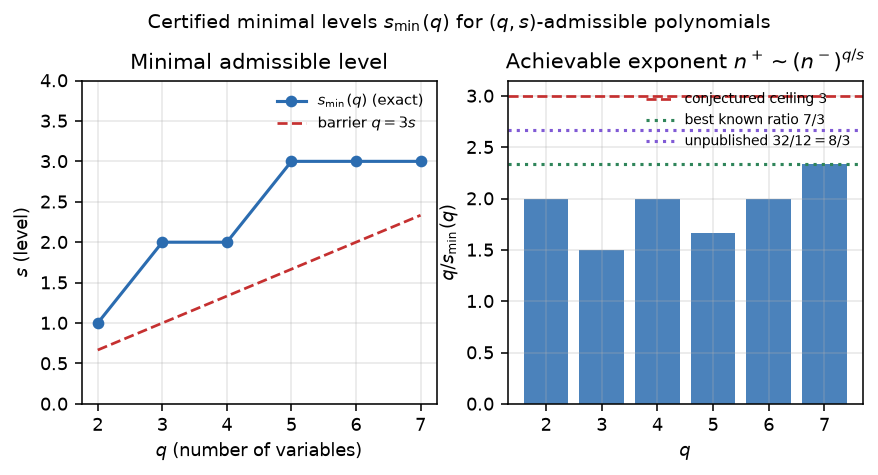
\includegraphics[width=\textwidth]{../figures/fig1_admissible_region.png}
\caption{Certified minimal levels $s_{\min}(q)$ (left) and the attainable exponent
$q/s_{\min}(q)$ (right).  The dashed line $q=3s$ is the barrier conjectured in
\textup{Conj.~\ref{conj:barrier}}; the certified data never reaches it.}
\label{fig:1}
\end{figure}

\subsection{Inertia growth and the coefficient profile}

\begin{figure}
\centering
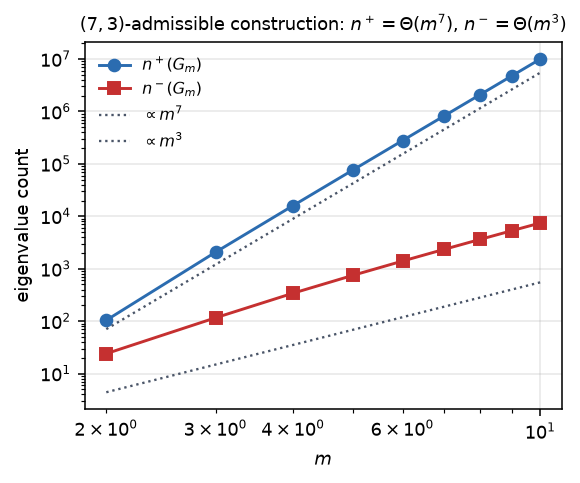
\includegraphics[width=0.45\linewidth]{../figures/fig2_inertia_growth.png}%
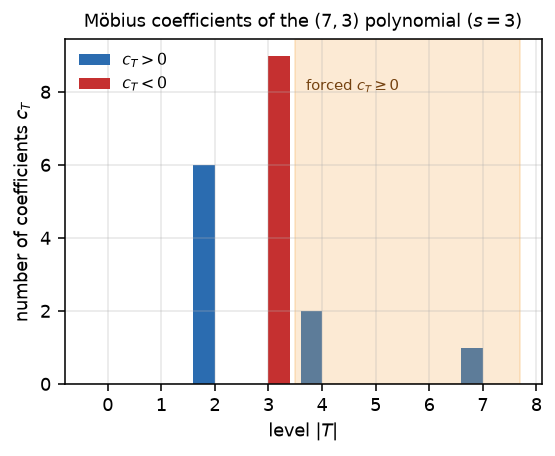
\includegraphics[width=0.45\linewidth]{../figures/fig3_coefficient_profile.png}
\caption{Left: $\pp$ and $n^-$ of the $(7,3)$ construction grow like $m^7$ and $m^3$.
Right: the level profile of the Moebius coefficients $c_T$; negatives are confined to
levels $\le 3$, which is exactly condition (c).}
\label{fig:2}
\end{figure}

Figure~\ref{fig:2} (left) is a log--log plot of the closed form of
Thm.~\ref{thm:spectrum}; it illustrates that the exponent $q/s$ really does manifest as
an exponent of $n^-$.  Figure~\ref{fig:2} (right) shows the coefficient profile: all
negatives live at levels $1$ and $3$, while $c_{[7]}=1$ forces the top level positive.

\subsection{Negative results}

We report two things that did not work.
\begin{itemize}
\item \textbf{We found no admissible pair with $q\ge3s$,} hence no improvement on the
      exponent $7/3$ (or on the $8/3$ reported in \cite{ElphickEtAl2026Inertia}).
      A local search over $g$ with the objective
      $\sum_{|T|>s}\max(0,1-c_T)+4\max(0,1-c_{[q]})$ drives the violation count to its
      floor $4$ on the boundary $q=3s$, i.e.\ it finds $g$ with all top-level $c_T\ge0$
      but $c_{[q]}=0$ rather than $\ge1$; making the last condition hold appears to be the
      real difficulty.
\item \textbf{Generalising $W(k)$ to Kneser graphs on $r$-subsets fails.}  One is tempted to
      replace the $2$-subsets in $W(k)$ by $r$-subsets, hoping for $\pp=\binom{k}{r}$
      and hence an exponential construction.  This does not work, and the reason is a
      small algebraic trap: for the incidence matrix $C$ of $r$-subsets,
      $K=J_N+(r-1)I_N-C^{\mathsf T}C$ is the Kneser adjacency matrix \emph{only for
      $r=2$}, because for $S\ne T$ with $|S\cap T|=t$ that expression has entry $1-t$
      rather than $\mathbf 1_{t=0}$.  For $r=3$, $k=6$ the resulting graph has inertia
      $(37,0,55)$ rather than the predicted $(84,9,0)$-type values, and the predicted
      $\pp=\binom kr$ would contradict (1): the $b$-vertices form an independent set of
      size $\binom kr$, so (1) forces $\pp\le k$.
\end{itemize}

\section{Limitations}

\begin{enumerate}
\item \textup{Conj.~\ref{conj:barrier}} is not proved.  The certified evidence covers
      $q\le7$; for $8\le q\le12$ we have uncertified values, and beyond that the
      $0$--$1$ program is out of reach for our solver.
\item We do not improve on the best exponent in the literature ($7/3$ published,
      $8/3$ reported).  Elphick--Kumar--Pragada--Spier note that to improve their result
      one must find a $(q,s)$-admissible polynomial with larger $q/s$; we have not done so.
\item Thm.~\ref{thm:s1} settles only $s=1$.  The certified table shows $s=2$ occurs for
      $q\in\{3,4\}$ and $s=3$ for $q\in\{5,6,7\}$, but a classification for fixed small $s$
      with unbounded $q$ is out of reach.
\item Exact characteristic polynomials are limited to order $\le40$; beyond that we rely on
      exact trace moments, which is a complete certificate of the spectrum but does not
      by itself exhibit it.
\item Our search is not exhaustive over the relevant family.  Milp feasibility with
      $2^q$ variables is notoriously hard, and a ``not found'' verdict is evidence only.
\end{enumerate}

\section{Conclusion and future work}

Admissibility of a Boolean polynomial with respect to its Moebius coefficients is the
compact object that controls how fast $\pp(G)$ may grow relative to $n^-(G)$.  We gave an
exact linearisation of that notion, settled its $s=1$ case completely, produced certified
exact data for $q\le7$, and formulated the sharp question of whether the exponent $q/s$ is
confined below $3$.

The most promising directions we can see are: (i) prove or refute
\textup{Conj.~\ref{conj:barrier}}, which would settle the currently open question of
whether $\pp$ admits any polynomial bound in $n^-$; (ii) exploit the recursion
$c_{T\cup\{q\}}=\widehat{g_1}(T)$, $c_T=\widehat{g_0}(T)-\widehat{g_1}(T)$ obtained by
splitting $g$ along the last coordinate, which suggests a divide-and-conquer search for
admissible $g$; (iii) classify admissible $g$ for fixed small $s$ and large $q$, the
complement of what we do here.

\begin{thebibliography}{9}

\bibitem[Akbari et al.]{AkbariEtAl2026}
S.~Akbari, C.~Elphick, H.~Kumar, S.~Pragada, Q.~Tang,
\emph{A new conjecture on the inertia of graphs}, Discrete Math.\ \textbf{349} (2026)
114953; arXiv:2508.01163.

\bibitem[Elphick et~al.]{ElphickEtAl2026Inertia}
C.~Elphick, H.~Kumar, S.~Pragada, T.~J.~Spier,
\emph{Resolution of a problem of Mohar on non-positive inertia}, arXiv:2609.06319 (2026).

\bibitem[Chen and Li]{ChenLi2026}
H.~Chen, J.~Li, \emph{Counterexamples to a conjecture on graph inertia}, arXiv:2605.07196
(2026).

\bibitem[Francis and Uptain]{FrancisUptain2026}
L.~Francis, T.~Uptain, \emph{The signature of connected line graphs is unbounded},
arXiv:2607.22874 (2026).

\bibitem[Cvetovi\'c, Doob and Sachs]{CvetkovicDoobSachs1980}
Z.~Cvetovi\'c, M.~Doob, H.~Sachs, \emph{Spectra of Graphs: Theory and Application},
Academic Press, 1980.

\bibitem[Brouwer and Haemers]{BrouwerHaemers2012}
A.~E.~Brouwer, W.~H.~Haemers, \emph{Spectra of Graphs}, Universitext, Springer, 2012.

\bibitem[Ma, Yang and Li]{MaYangLi2013}
W.~Ma, W.~Yang, S.~Li, \emph{Positive and negative inertia index of a graph}, Linear
Algebra Appl.\ \textbf{438} (2013) 331--341.

\bibitem[Fan and Wang]{FanWang2017}
Y.-Z.~Fan, L.~Wang, \emph{Bounds for the positive and negative inertia index of a graph},
Linear Algebra Appl.\ \textbf{522} (2017) 15--27.

\bibitem[Xu, Zhen and Wong]{XuZhenWong2024}
S.~Xu, W.~Zhen, D.~Wong, \emph{The relationship between the negative inertia index of
graph $G$ and its girth $g$ and diameter $d$}, arXiv:2312.02680 (2023).

\bibitem[Delsarte, Goethals and Seidel]{DelsarteGoethalsSeidel1978}
P.~Delsarte, J.~M.~Goethals, J.~J.~Seidel, \emph{Spherical codes and designs},
Geom.\ Dedicata \textbf{6} (1978) 363--388.

\bibitem[Torga{\v{s}}ev(a)]{Torgasev1985a}
J.~Torga{\v{s}}ev, \emph{On graphs with a fixed number of negative eigenvalues}, Discrete
Math.\ \textbf{57} (1985) 311--317.

\bibitem[Torga{\v{s}}ev(b)]{Torgasev1985b}
J.~Torga{\v{s}}ev, \emph{Graphs with exactly two negative eigenvalues}, Math.\ Nachr.\
\textbf{122} (1985) 135--140.

\bibitem[Torga{\v{s}}ev(c)]{Torgasev1989}
J.~Torga{\v{s}}ev, \emph{Maximal canonical graphs with three negative eigenvalues},
Publ.\ Inst.\ Math.\ (Belgr.) \textbf{45}(59) (1989) 7--10.

\bibitem[Torga{\v{s}}ev(d)]{Torgasev1992}
J.~Torga{\v{s}}ev, \emph{On the numbers of positive and negative eigenvalues of a graph},
Publ.\ Inst.\ Math.\ (Belgr.) \textbf{51}(65) (1992) 25--28.

\bibitem[Kotlov and Lov\'asz]{KotlovLovasz1996}
V.~Kotlov, L.~Lov\'asz, \emph{The rank and size of graphs}, J.\ Graph Theory \textbf{23}
(1996) 185--189.

\bibitem[Barrett et~al.]{BarrettEtAl2014}
W.~Barrett, S.~Butler, M.~Catral, M.~S.~Fallat, H.~T.~Hall, L.~Hogben, M.~Young,
\emph{The principal rank characteristic sequence over various fields}, Linear Algebra
Appl.\ \textbf{459} (2014) 222--236.

\bibitem[Cvetovi\'ic]{Cvetkovic1971}
Z.~Cvetovi\'ic, \emph{Graphs and their spectra}, Publ.\ Elektrotehn.\ Fak.\ Ser.\ Mat.\
Fiz. (354--356) (1971) 1--50.

\bibitem[Cvetovi\'ic and Simi\'c]{CvetkovicSimic1993}
Z.~Cvetovi\'ic, S.~Simi\'c, \emph{Non-complete extended $P$-sum of graphs, graph angles
and star partitions}, Publ.\ Inst.\ Math.\ (Beograd) (N.S.) \textbf{53}(67) (1993)
4--16.

\bibitem[Hardy, Littlewood and P\'olya]{HardyLittlewoodPolya1952}
G.~H.~Hardy, J.~E.~Littlewood, G.~P\'olya, \emph{Inequalities}, 2nd ed., Cambridge
Univ.\ Press, 1952.

\bibitem[Courant and Fischer]{CourantFischer1927}
R.~Courant, H.~Fischer, \emph{\\"Uber die Eigenwerte symmetrischer Matrizen}, Math.\ Ann.\
\textbf{97} (1927) 621--630.

\bibitem[Hoffman]{Hoffman1947}
K.~Hoffman, \emph{The construction of least squares multivariate polynomials}, Ann.\ Math.\
Statist.\ \textbf{18} (1947) 766--772.

\bibitem[SciPy]{SciPy2020}
P.~Virtanen et~al., \emph{SciPy 1.0: fundamental algorithms for scientific computing in
Python}, Nature Methods \textbf{17} (2020) 261--272.

\bibitem[SymPy]{SymPy2011}
A.~M.~S.~Palmer et~al., \emph{SymPy: symbolic computing in Python}, Proc.\ SciPy 2011.

\bibitem[HiGHS]{HuangfuHall2018}
Q.~Huangfu, J.~A.~J.~Hall, \emph{Parallelizing the dual revised simplex method}, Math.\
Program.\ Comput. \textbf{10} (2018) 119--142.

\bibitem[NetworkX]{NetworkX2020}
A.~Hagberg, P.~J.~Swart, D.~A.~Livingston, R.~Kenny, \emph{NetworkX: network analysis and
toolbox in Python}, Proc.\ SciPy 2020.

\end{thebibliography}

\end{document}